\documentclass[12pt]{article}
%\usepackage[margin=1in]{geometry}
\usepackage[left=2.5cm, right=2.5cm, top=2cm]{geometry}
\usepackage{amsmath, amsthm, amssymb, amsfonts}
\usepackage{scrextend}
\usepackage{graphicx}
\usepackage{multicol}
\usepackage{hyperref}


% Set up stuff to handle Python code nicely.
\usepackage{listings}
\usepackage{color}

\definecolor{codegreen}{rgb}{0,0.6,0}
\definecolor{codegray}{rgb}{0.5,0.5,0.5}
\definecolor{codepurple}{rgb}{0.58,0,0.82}
\definecolor{backcolour}{rgb}{0.95,0.95,0.92}

\lstdefinestyle{mystyle}{
    backgroundcolor=\color{backcolour},
    commentstyle=\color{codegreen},
    keywordstyle=\color{magenta},
    numberstyle=\tiny\color{codegray},
    stringstyle=\color{codepurple},
    basicstyle=\footnotesize,
    breakatwhitespace=false,
    breaklines=true,
    captionpos=b,
    keepspaces=true,
    numbers=left,
    numbersep=5pt,
    showspaces=false,
    showstringspaces=false,
    showtabs=false,
    tabsize=2
}

\lstset{style=mystyle}

\setlength{\columnsep}{0.3in}

\newcommand{\N}{\mathbb{N}}
\newcommand{\Z}{\mathbb{Z}}

\newenvironment{problem}[2][Problem]{\begin{trivlist}
\item[\hskip \labelsep {\bfseries #1}\hskip \labelsep {\bfseries #2.}]}{\end{trivlist}}
%If you want to title your bold things something different just make another thing exactly like this but replace "problem" with the name of the thing you want, like theorem or lemma or whatever

\newenvironment{answer}[2][Answer]{\begin{trivlist}
\item[\hskip \labelsep {\bfseries #1}\hskip \labelsep {\bfseries #2.}]}{\end{trivlist}}

\newcommand\textlcsc[1]{\textsc{\MakeLowercase{#1}}}

% Enable one-column figures in multicol.
\newenvironment{Figure}
  {\par\medskip\noindent\minipage{\linewidth}}
  {\endminipage\par\medskip}


\begin{document}

%\renewcommand{\qedsymbol}{\filledbox}
%Good resources for looking up how to do stuff:
%Binary operators: http://www.access2science.com/latex/Binary.html
%General help: http://en.wikibooks.org/wiki/LaTeX/Mathematics
%Or just google stuff

% \title{AST 221: Problem Set 1}
% \author{Jonas Powell}
% \maketitle


% make title bold and 14 pt font (Latex default is non-bold, 11 pt)
\title{\Large \textbf{Galactic Astronomy: Problem Set 4}}

\author{{\rm Jonas Powell, \textit{Wesleyan University}}}


\maketitle


\begin{addmargin}[4em]{4em}
\noindent {\bf Due: Thursday, April 4 by midnight.} Late papers are not accepted after April 4 (midnight). If you cannot complete the assignment, hand in what you have completed before the deadline. Consider the deadline to be like the boarding time for an airplane, or the deadline for a grant submission to NASA or NSF. If you miss the deadline, you do not get on the airplane, no matter how good your excuse is. If you miss an NSF or NASA deadline, you do not get the grant, no matter how good your project is. The best advice is ... finish early. You can submit multiple times, right up to the deadline. Whatever your latest submission is, when the deadline occurs, is what will be graded.
\bigskip \bigskip
\end{addmargin}


% Begin two-column layout
% if using this, change margins (line 3) to like 1cm-ish
%\begin{multicols*}{2}

% A FIGURE
% \begin{figure}[htp]
%   \hspace*{\fill}%
%   \subcaptionbox{\label{fig:lab2}}{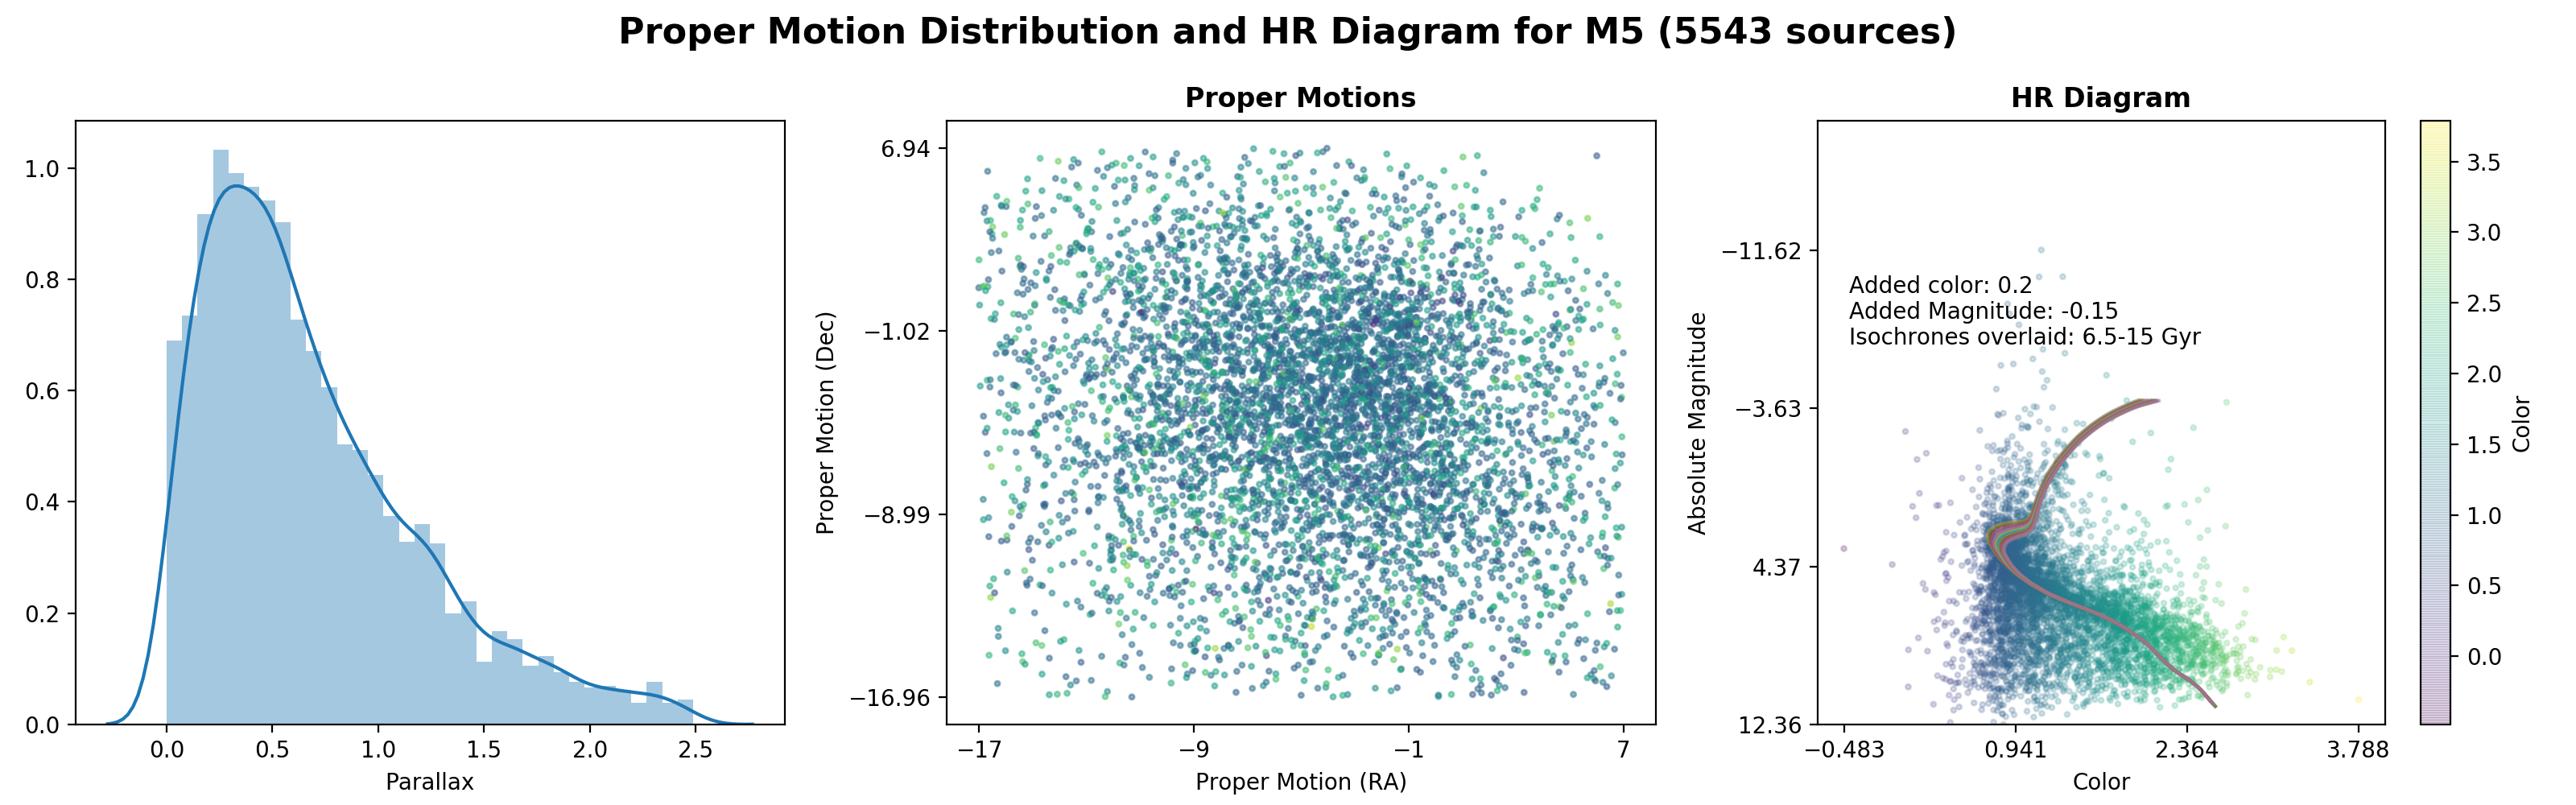
\includegraphics[width=0.48\linewidth]{HRD_M5_7000.png}}\hfill%
%   \subcaptionbox{\label{fig:lab2}}{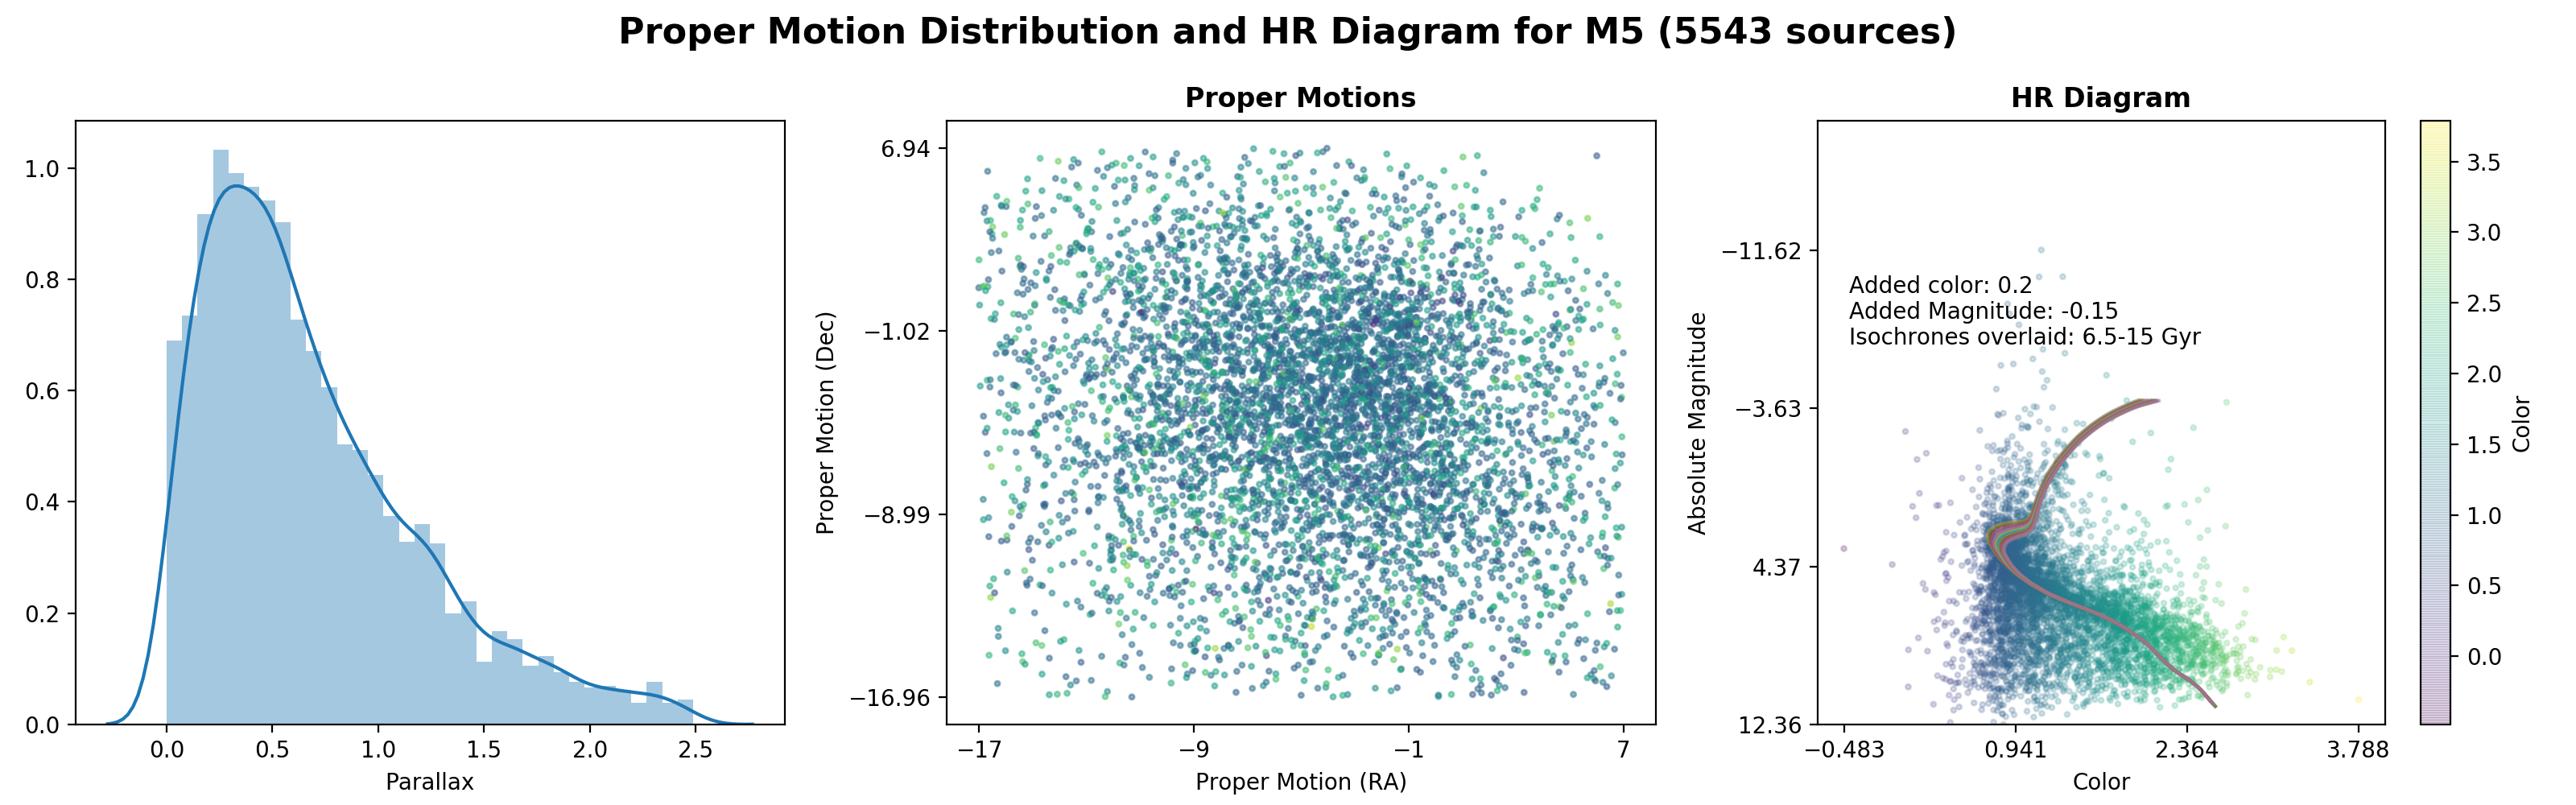
\includegraphics[width=0.48\linewidth]{HRD_M5_7000.png}}\hfill%
%   \hspace*{\fill}%
%   \caption{blah}
% \end{figure}


\begin{problem}{1 \& 2}
  Make an HR diagram of an open (galactic) cluster based on the Gaia catalogue. You may choose any cluster EXCEPT the Pleiades (since you already did the Pleiades as an exercise last semester in AST 222). Also, please make sure you have made a UNIQUE choice of galactic cluster -- do not use the same cluster as any other classmate. (I suggest posting a cluster sign-up board in the student office to be sure that no one duplicates another person's cluster). You can adjust several parameters in selecting members, including the exact position of the center of your search area and the size of your search box. You can use parallaxes and/or kinematic information (proper motions and/or space motions) to help eliminate field stars. Your objective is to get as clean an HR diagram of your cluster as possible -- ie. containing enough cluster members to clearly define the cluster HR diagram with as few non-members as possible. Do NOT remove stars arbitrarily from the diagram just because they don't fit your pre-conceived notion of what the HR diagram should look like! (That's a bad practice in science ...).

  Once you have a nice cluster HR diagram, overlay on it a ZAMS with the metallicity appropriate to the cluster. You can use the Dartmouth Stellar Evolution Data Base (linked on the course Moodle page) to obtain model results in the Gaia magnitude system. For the galactic cluster, you can use a metallicity of 0 -- i.e. solar. If it is a globular cluster, you will need to look up the metallicity of the cluster and choose an appropriate ZAMS. Adjust the horizontal location of the ZAMS to account for the foreground reddening of the cluster (which you will have to look up or figure out yourself). Then adust the vertical location of the ZAMS to match the cluster MS and use the amount of adjustment to calculate the distance to the cluster.

\end{problem}


\begin{answer}{1 \& 2}

  Presented here are plots for Messier 42, or The Orion Nebula. The code that created these plots is attached at the end of the problem set.


  \begin{figure}[htp]
    \hspace*{\fill}%
    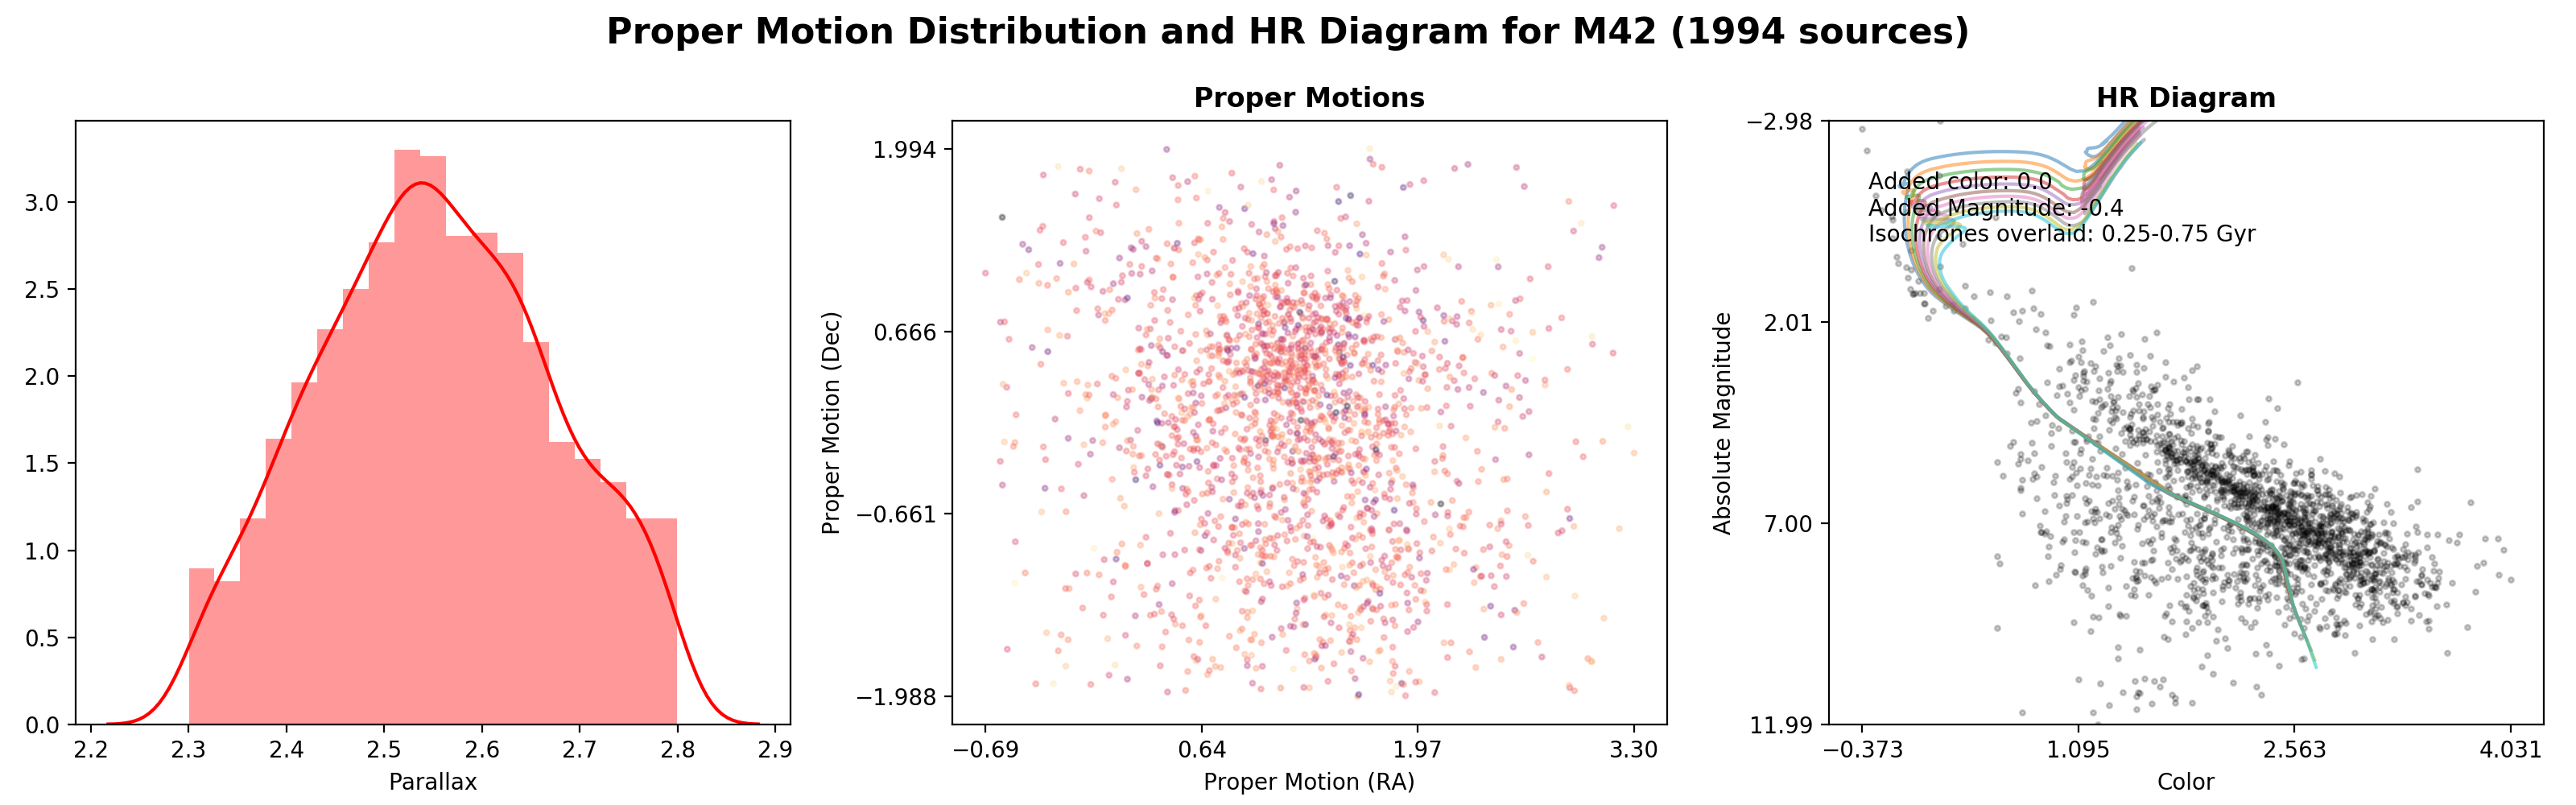
\includegraphics[width=0.98\linewidth]{HRD_M42_70000.png}}\hfill%
    \hspace*{\fill}%
    \caption{\textit{Left, Center}: Plots of the M42 sample's distribution in parallax and proper motion space, used as checks on the validity of the regional cuts made to isolate the cluster. \textit{Right}: M42's HR diagram, overlaid with some isochrones.}
  \end{figure}


\end{answer}
\bigskip \bigskip




\begin{problem}{3}
  Repeat the process in Problems 1 and 2 for a globular cluster of your choice. Again, please make sure your choice of globular cluster is unique.
\end{problem}

\begin{answer}{3}

  Presented here are plots for NGC104, or $\xi$ Tucanae. The code that created these plots is attached at the end of the problem set.

\begin{answer}{1 \& 2}
  \begin{figure}[htp]
    \hspace*{\fill}%
    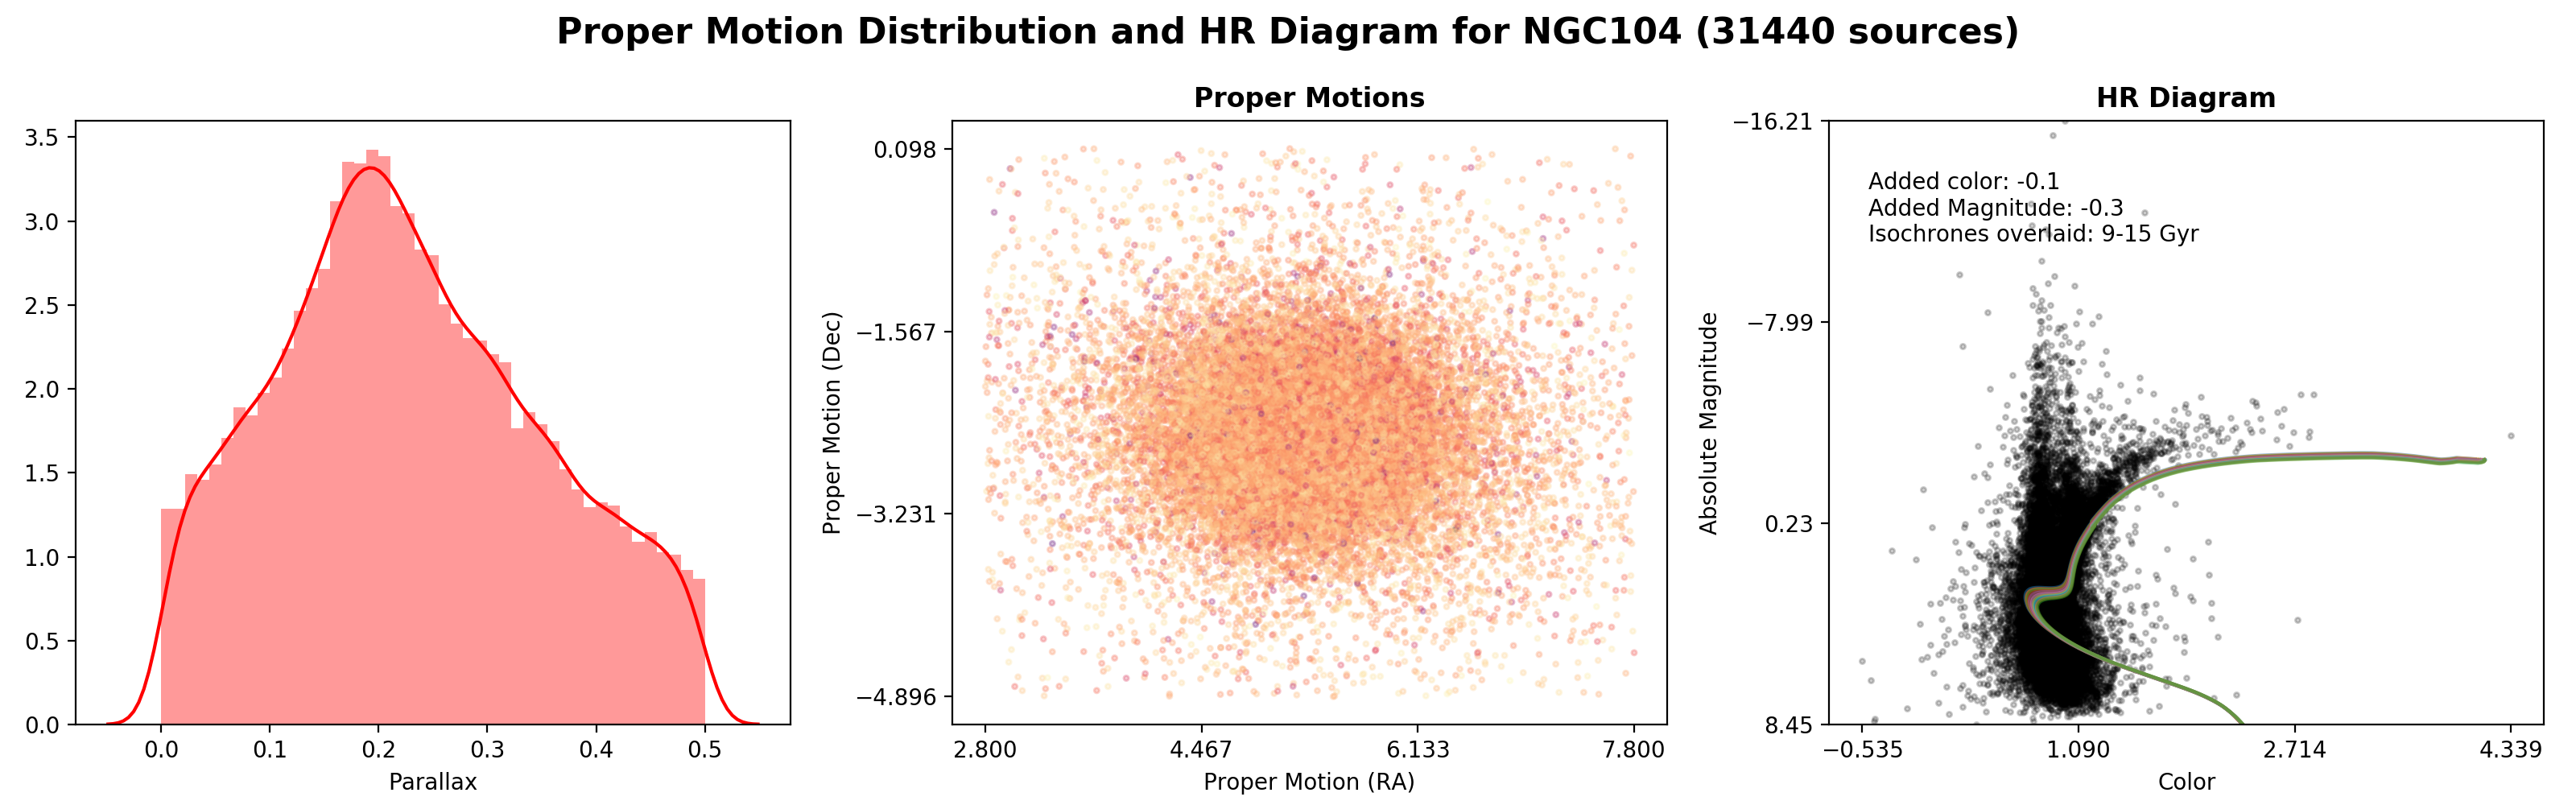
\includegraphics[width=0.98\linewidth]{HRD_NGC104_70000.png}}\hfill%
    \hspace*{\fill}%
    \caption{\textit{Left, Center}: Plots of the NGC104 sample's distribution in parallax and proper motion space, used as checks on the validity of the regional cuts made to isolate the cluster. \textit{Right}: NGC104's HR diagram, overlaid with some isochrones.}
  \end{figure}

\end{answer}
\bigskip \bigskip



\begin{problem}{4}
   Discuss the HR diagrams above and your procedures for obtaining them. What features can you clearly see on each figure. Identify well known features such as the MS turnoff, the RG, HB, AGB features and the presence or absence of WDs. Can you see a binary sequence? Can you see blue stragglers? Can you see supergiants? Comment on any other aspects of the HR diagram or the procedure for selecting members and non-members that you find noteworthy.
\end{problem}

\begin{answer}{4}



To get these data, I developed a Python \texttt{class} object that retrieved Gaia data and the isochrone tracks. The Gaia data were retrieved using \texttt{astroquery}'s Gaia querier in SQL. Cuts were made in position, proper motion, and parallax spaces, usually with tolerances (i.e. boxes around the central point) of around half a degree for position, 3 km s$^{-1}$ for proper motions, and 1-3 degrees for parallax.

Very rough isochrone fitting indicated that M42 is in the 0.25-0.75 Gyr range, while NGC104 is between 9-15 Gyr, both of which consistent with the literature values of around 0.3 and 13 Gyr, respectively.

As the annotations on the HR diagrams show, horizontal (color) offsets of 0 and -0.1 were added for M42 and NGC104, respectively, while vertical (magnitude) offsets were -0.4 and -0.3.

Since I chose to put my HR diagram on an absolute-magnitude scale (since we know the parallax of these sources, the conversion becomes quite trivial), the magnitude corrections needed for the isochrones were not significant and generally hovered around zero. However, if I were to put my HR diagram on an apparent magnitude scale, I would be able to calculate the distance to the cluster by using familiar distance modulus and rearranging it for distance:

\begin{align*}
  m - M &= 5\log_{10} (\frac{d}{10}) \\
  \rightarrow d &= 10 \times (100^{(m - M)/5})^2 \text{ parsecs} \\
\end{align*}

We can actually do this backwards, using the first of the equations, and find that I would have had to shift the isochrone by about eight magnitudes to compensate for M42's distance of 389 parsecs, while NGC104, at 4kpc, would have required 13 magnitudes of compensation.



I was surprised to find that my cuts did not yield particularly clean data, as is shown in the plots attached. While the general stellar tracks can more or less be seen, it is strange to me that there are still so many field stars. Still, the plots certainly have sufficient detail to locate familiar features: in M42's HR diagram, we can see that, if we anchor the isochrone at the Main Sequence turnoff, then the majority of what appears to be the Main Sequence actually reveals itself to be PMS stars that have not yet made it to the MS. In M42, as expected, there are no branch features, as the stars are far too young. Conversely, $\xi$ Tucanae's diagram tells a dramatically different story, with loads of branch stars and no main sequence presence (this time because they're all too old). The juxtaposition of extremely young and extremely old clusters in these two plots is fascinating.



\end{answer}









%\end{multicols*}
\vfill\eject
\clearpage


\lstinputlisting[language=Python]{get_cluster.py}
\lstinputlisting[language=Python]{scratch_hw4.py}



\end{document}
